\documentclass[11pt,a4paper]{article}
\usepackage[utf8]{inputenc}
\usepackage[T1]{fontenc}
\usepackage{array}
\usepackage{amsmath}
\usepackage{amsfonts}
\usepackage{siunitx}
\usepackage{placeins}
\usepackage{amssymb}
\usepackage{makeidx}
\usepackage{sidecap}
\usepackage{fvextra}
\usepackage{multicol}
\usepackage{listings}
\usepackage{appendix}
\usepackage{comment}
\usepackage{nicematrix}
\usepackage{multirow}
\usepackage{braket}
\usepackage{graphicx}
\usepackage{relsize}
\usepackage{fancyhdr}
\usepackage{cprotect}
\usepackage{color} 
\usepackage{hyperref}
\hypersetup{
	colorlinks=true, 
	linktoc=all, 
	linkcolor=blue,
	urlcolor=blue
}
\usepackage[left=2cm,right=2cm,top=1.5cm,bottom=2cm]{geometry}
\usepackage{titling}
\usepackage{etoolbox}
\flushbottom
\title{Statistical Analysis of Experimental Data\\
	\vspace{0.2cm}
	\large{Homework 04}}
\vspace{-0.2cm}
\author{Igor Di Tota}
\date{\small \url{https://github.com/igordt/SAED_homeworks/tree/main}}


\begin{document}
	\maketitle
	
	\section*{Introduction}
	
	This homework concerns the propagation of uncertainties: \textit{consider production of rectangular tables with length $L = 160$ cm and width $W = 90$ cm. Tolerance of production process (standard deviation) is $\sigma_L = 0.5$ cm for the table length and $\sigma_W = 0.3$ cm for the table width. Assuming length and width are independent random variables and table sides are always perpendicular:}
	\begin{enumerate}
		\item \textit{Calculate (from analytical formulae):}
		\begin{itemize}
			\item \textit{the expected variation (standard deviation) of the table surface,}
			\item \textit{the expected variation of the total length of the table sides,}
			\item \textit{the expected variation of the table diagonal,}
			\item \textit{the expected correlation between the surface and the total edge length.}
		\end{itemize}
		\item \textit{Perform numerical experiment generating table lengths and widths from the Gaussian distribution to calculate same parameters, compare results of the two approaches.}
	\end{enumerate}
	
	The quantities studied are
	\begin{equation}
		S = L\, W, \qquad P = 2(L + W), \qquad D = \sqrt{L^2 + W^2},
	\end{equation}
	that is the table surface, the total length of the table sides (perimeter) and the table diagonal.
	
	\section*{Analytical error propagation}
	
	The input variables are $\mathbf{X} = (L, W)$.
	Since length and width are independent, their covariance matrix is diagonal:
	\begin{equation}
		\mathbb{C}_X =
		\begin{pmatrix}
			\sigma_L^2 & 0 \\
			0 & \sigma_W^2
		\end{pmatrix}.
	\end{equation}
	The output variables are $\mathbf{Y} = (S, P, D)$.
	To propagate the uncertainties from $\mathbf{X}$ to $\mathbf{Y}$, the general error propagation formula seen in the lecture is used:
	\begin{equation}
		\mathbb{C}_Y = A\, \mathbb{C}_X\, A^\intercal ,
		\label{eq:propagation}
	\end{equation}
	where $A$ is the matrix of partial derivatives $A_{ij} = \partial y_i / \partial x_j$, evaluated at the nominal values $L = 160$ cm and $W = 90$ cm:
	\begin{equation}
		A =
		\begin{pmatrix}
			\dfrac{\partial S}{\partial L} & \dfrac{\partial S}{\partial W} \\[2ex]
			\dfrac{\partial P}{\partial L} & \dfrac{\partial P}{\partial W} \\[2ex]
			\dfrac{\partial D}{\partial L} & \dfrac{\partial D}{\partial W}
		\end{pmatrix}
		=
		\begin{pmatrix}
			W & L \\[1ex]
			2 & 2 \\[1ex]
			\dfrac{L}{D} & \dfrac{W}{D}
		\end{pmatrix}.
	\end{equation}
	
	Eq.~\eqref{eq:propagation} comes from a first order Taylor expansion of $\mathbf{Y}(\mathbf{X})$ around the nominal values, so it is only an approximation for non-linear functions such as $S$ and $D$, while it is exact for the perimeter $P$, which is linear in $L$ and $W$.
	The approximation is good when the standard deviations are small compared to the nominal values, as in this case ($\sigma_L / L \approx 0.3\%$, $\sigma_W / W \approx 0.3\%$).
	
	The relevant elements of $\mathbb{C}_Y$ are
	\begin{equation}
		\sigma_S^2 = W^2\sigma_L^2 + L^2\sigma_W^2, \qquad
		\sigma_P^2 = 4\left(\sigma_L^2 + \sigma_W^2\right), \qquad
		\sigma_D^2 = \frac{L^2\sigma_L^2 + W^2\sigma_W^2}{L^2 + W^2},
	\end{equation}
	\begin{equation}
		\mathrm{Cov}(S, P) = 2\left(W\,\sigma_L^2 + L\,\sigma_W^2\right),
	\end{equation}
	and the correlation coefficient between the surface and the total edge length is
	\begin{equation}
		\rho(S, P) = \frac{\mathrm{Cov}(S, P)}{\sigma_S\, \sigma_P}.
	\end{equation}
	The numerical values are reported in Table~\ref{tab:analytical}.
	
	\begin{table}[!h]
		\centering
		\begin{tabular}{l c c c}
			\hline
			Quantity & Nominal value & $\sigma$ & relative uncertainty \\
			\hline
			Surface $S$   & $14400.0$ cm$^2$ & $65.8$ cm$^2$ & $0.46\,\%$ \\
			Perimeter $P$ & $500.00$ cm      & $1.17$ cm     & $0.23\,\%$ \\
			Diagonal $D$  & $183.58$ cm      & $0.46$ cm     & $0.25\,\%$ \\
			\hline
		\end{tabular}
		\caption{Nominal values and standard deviations of the surface, perimeter and diagonal of the table, obtained from the analytical error propagation.}
		\label{tab:analytical}
	\end{table}
	\FloatBarrier
	
	The covariance and the correlation coefficient between the surface and the perimeter are
	\begin{equation}
		\mathrm{Cov}(S, P) = 73.80 \ \text{cm}^3, \qquad \rho(S, P) = 0.9618 .
	\end{equation}
	
	\subsection*{Comments on the analytical results}
	
	\paragraph{Surface.} The surface has the largest relative uncertainty.
	As shown in the lecture, for a product of independent variables the relative uncertainties add in quadrature:
	\begin{equation}
		\frac{\sigma_S}{S} = \sqrt{\left(\frac{\sigma_L}{L}\right)^2 + \left(\frac{\sigma_W}{W}\right)^2} = \sqrt{(0.31\%)^2 + (0.33\%)^2} \approx 0.46\% .
	\end{equation}
	The two contributions are comparable: $W^2\sigma_L^2 = 2025 \ \text{cm}^4$ and $L^2\sigma_W^2 = 2304 \ \text{cm}^4$.
	
	\paragraph{Perimeter.} For a sum the absolute uncertainties add in quadrature, so $\sigma_P = 2\sqrt{\sigma_L^2 + \sigma_W^2}$.
	Since $P$ is linear in $L$ and $W$, this result is exact and not an approximation.
	
	\paragraph{Diagonal.} The variance of the diagonal is dominated by the length: $L^2\sigma_L^2 = 6400 \ \text{cm}^4$ against $W^2\sigma_W^2 = 729 \ \text{cm}^4$, so about $90\%$ of $\sigma_D^2$ comes from $L$.
	This is expected, since the diagonal of a long table is almost parallel to its longer side.
	
	\paragraph{Correlation.} The correlation between $S$ and $P$ is very strong and positive, $\rho(S, P) \approx 0.96$: both quantities increase when $L$ or $W$ increase, so they fluctuate together.
	
	\section*{Numerical experiment}
	
	To check the analytical results, the production of $N = 10^6$ tables is simulated.
	For each table, the length and the width are drawn independently from Gaussian distributions:
	\begin{equation}
		L_i \sim \mathcal{N}(L, \sigma_L^2), \qquad W_i \sim \mathcal{N}(W, \sigma_W^2), \qquad i = 1, \dots, N ,
	\end{equation}
	and the surface $S_i$, the perimeter $P_i$ and the diagonal $D_i$ are computed.
	
	\subsection*{Sample variance}
	
	Let $x_1, \dots, x_N$ be one of these samples, coming from a distribution with true mean $\mu$ and true variance $\sigma^2$.
	The true mean is estimated with the sample mean $\bar{x} = \frac{1}{N} \sum_i x_i$, which has variance $\mathbb{V}(\bar{x}) = \sigma^2 / N$.
	To measure the spread of the sample, the deviation of each value from the sample mean, $x_i - \bar{x}$, is taken and the squared deviations are averaged:
	\begin{equation}
		d^2 = \frac{1}{N} \sum_i (x_i - \bar{x})^2 .
	\end{equation}
	$d^2$ is a biased estimator of $\sigma^2$.
	Writing each deviation as $x_i - \bar{x} = (x_i - \mu) - (\bar{x} - \mu)$ and expanding the square:
	\begin{equation}
		\begin{aligned}
			d^2 &= \frac{1}{N} \sum_i \left[ (x_i - \mu)^2 - 2 (x_i - \mu)(\bar{x} - \mu) + (\bar{x} - \mu)^2 \right] \\
			&= \frac{1}{N} \sum_i (x_i - \mu)^2 - 2 (\bar{x} - \mu) \underbrace{\frac{1}{N} \sum_i (x_i - \mu)}_{=\ \bar{x} - \mu} + (\bar{x} - \mu)^2 \\
			&= \frac{1}{N} \sum_i (x_i - \mu)^2 - (\bar{x} - \mu)^2 .
		\end{aligned}
	\end{equation}
	Taking the expectation value, the first term gives $\sigma^2$ and the second one gives the variance of the sample mean:
	\begin{equation}
		\langle d^2 \rangle = \sigma^2 - \mathbb{V}(\bar{x}) = \sigma^2 - \frac{\sigma^2}{N} = \frac{N-1}{N}\, \sigma^2 .
	\end{equation}
	To correct this bias, $d^2$ is multiplied by Bessel's factor $N / (N-1)$, which gives the sample variance\footnote{In \texttt{numpy}, the sample standard deviation $s$ is computed with \texttt{x.std(ddof=1)}, where \texttt{ddof} is subtracted from $N$ in the denominator.}
	\begin{equation}
		s^2 = \frac{N}{N-1}\, d^2 = \frac{1}{N-1} \sum_i (x_i - \bar{x})^2 , \qquad \langle s^2 \rangle = \sigma^2 .
	\end{equation}
	
	\subsection*{Sample correlation}
	
	In the same way, the correlation between $S$ and $P$ is estimated with the sample covariance and the sample correlation coefficient:
	\begin{equation}
		s^2_{SP} = \frac{1}{N-1} \sum_i (S_i - \bar{S})(P_i - \bar{P}), \qquad r_{SP} = \frac{s^2_{SP}}{s_S\, s_P} ,
	\end{equation}
	where $s_S$ and $s_P$ are the sample standard deviations of $S$ and $P$.
	
	As a check of the generation, the generated inputs have sample means $\bar{L} = 159.9995$ cm and $\bar{W} = 90.0004$ cm, and sample standard deviations $s_L = 0.4998$ cm and $s_W = 0.2999$ cm, in agreement with the nominal values.
	
	\section*{Comparison of the two approaches}
	
	The analytical and numerical results are compared in Table~\ref{tab:comparison}.
	To quantify the agreement, for each quantity the relative difference between the numerical estimate and the analytical value is computed:
	\begin{equation}
		\Delta_{\text{rel}} = \frac{x_{\text{num}} - x_{\text{an}}}{x_{\text{an}}} .
	\end{equation}
	
	\begin{table}[!h]
		\centering
		\begin{tabular}{l c c c}
			\hline
			Quantity & Analytical & Numerical & $\Delta_{\text{rel}}$ \\
			\hline
			$\sigma_S$ [cm$^2$]       & $65.7951$ & $65.7891$ & $-0.009\,\%$ \\
			$\sigma_P$ [cm]           & $1.1662$  & $1.1660$  & $-0.014\,\%$ \\
			$\sigma_D$ [cm]           & $0.4599$  & $0.4598$  & $-0.021\,\%$ \\
			$\mathrm{Cov}(S, P)$ [cm$^3$] & $73.8000$ & $73.7847$ & $-0.021\,\%$ \\
			$\rho(S, P)$              & $0.9618$  & $0.9618$  & $+0.003\,\%$ \\
			\hline
		\end{tabular}
		\caption{Comparison between the analytical results and the numerical estimates obtained from $N = 10^6$ simulated tables.}
		\label{tab:comparison}
	\end{table}
	\FloatBarrier
	
	To judge whether these differences are significant, the statistical uncertainty of the numerical estimates, which are obtained from a finite sample, is needed.
	For a Gaussian variable, the relative uncertainty on the sample standard deviation can be estimated in three steps:
	\begin{enumerate}
		\item for large $N$, the sample variance $s^2$ is essentially the mean of the $N$ independent squared deviations $y_i = (x_i - \mu)^2$, whose mean value is $\sigma^2$;
		\item as shown in the lecture, the standard deviation of a mean of $N$ independent values is the standard deviation of a single value divided by $\sqrt{N}$; for a Gaussian variable the squared deviations $y_i$ have standard deviation $\sqrt{2}\,\sigma^2$, so
		\begin{equation}
			\frac{\sigma(s^2)}{s^2} \approx \frac{\sqrt{2}\,\sigma^2}{\sqrt{N}\,\sigma^2} = \sqrt{\frac{2}{N}} ;
		\end{equation}
		\item the standard deviation is $s = (s^2)^{1/2}$ and, as follows from error propagation, for a power the relative uncertainty is multiplied by the exponent, here $1/2$:
		\begin{equation}
			\frac{\sigma(s)}{s} \approx \frac{1}{2}\sqrt{\frac{2}{N}} = \frac{1}{\sqrt{2N}} \approx 0.07\% \qquad \text{for } N = 10^6 .
		\end{equation}
	\end{enumerate}
	This holds for Gaussian variables; $S$ and $D$ are not exactly Gaussian, but with relative tolerances of $\approx 0.3\%$ they are very close to it.
	All the observed differences on the standard deviations are therefore well within the statistical precision of the simulation; the same holds for the covariance and the correlation coefficient.
	
	The agreement confirms that:
	\begin{itemize}
		\item for the perimeter $P$, which is linear in $L$ and $W$, the propagation formula is exact;
		\item for the surface $S$ and the diagonal $D$, which are non-linear, the first order approximation is enough, since the effect of the neglected higher order terms on the standard deviations is far below the statistical precision of the simulation;
		\item the sample correlation coefficient $r_{SP}$ estimated from the simulated tables agrees with the analytical correlation $\rho(S, P) \approx 0.96$, with a relative difference of only $0.003\%$.
	\end{itemize}
	
	\section*{Visualisation of the generated tables}
	
	To visualise the effect of the production tolerances, the first 10 generated tables are drawn with the bottom-left corner fixed at the origin (Figure~\ref{fig:tables}).
	Since the fluctuations are of a few millimetres, a zoom on the top-right corner is also shown, in a range of $\pm 3\sigma$ around the nominal dimensions.
	
	\begin{figure}[!h]
		\centering
		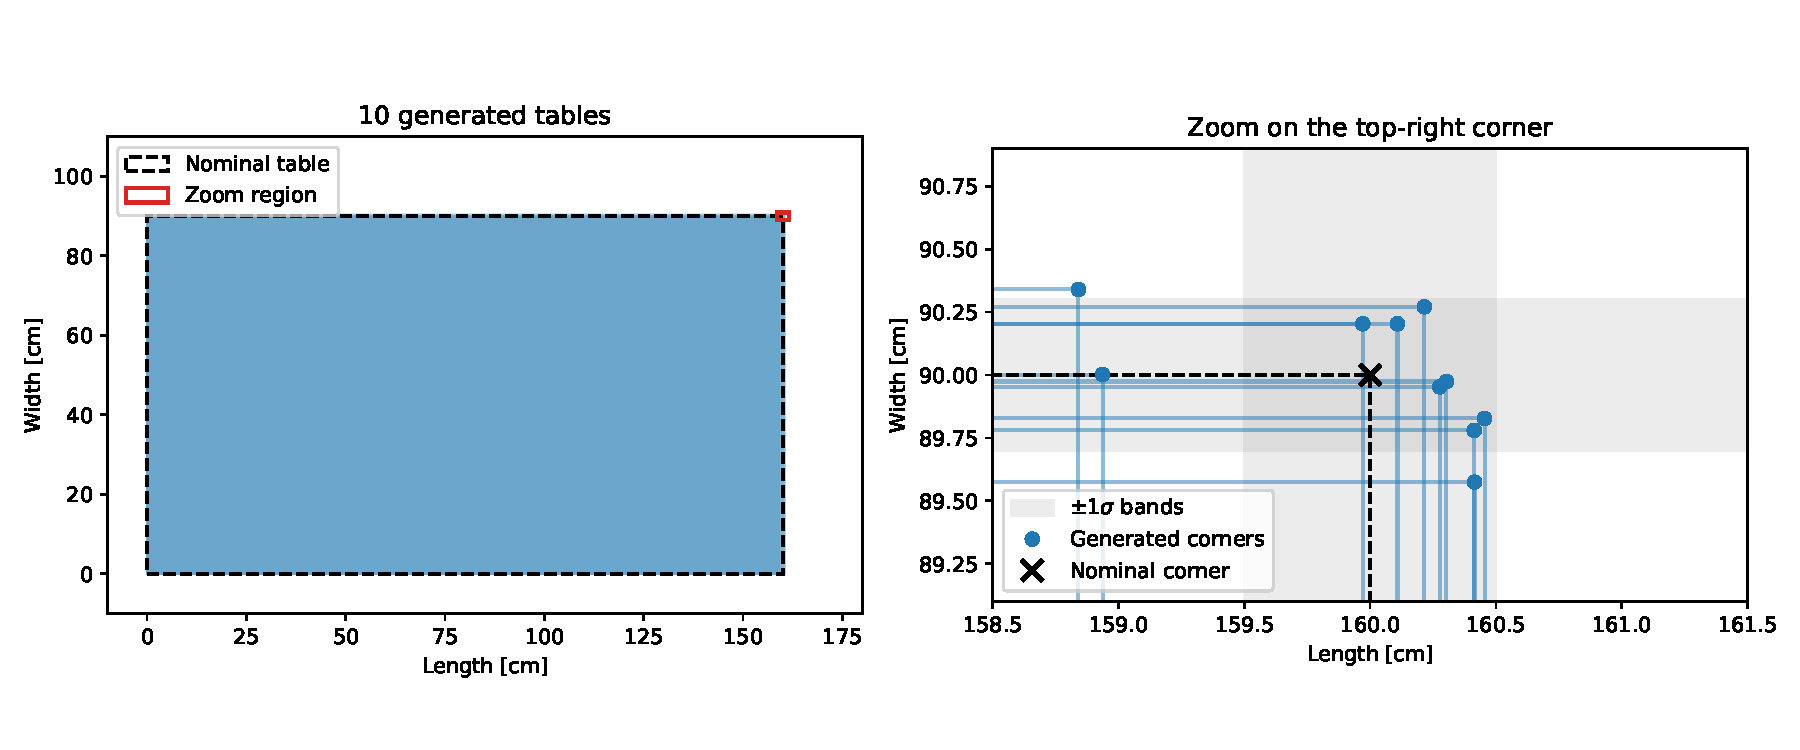
\includegraphics[width=\linewidth]{images/tables.pdf}
		\caption{Left: the first 10 generated tables, with the bottom-left corner fixed at the origin; the dashed line is the nominal table and the red box marks the zoomed region. Right: zoom on the top-right corner, with the corners of the generated tables, the nominal corner and the $\pm 1\sigma$ intervals of $L$ and $W$ (green bands).}
		\label{fig:tables}
	\end{figure}
	\FloatBarrier
	
	\section*{Distributions of the derived quantities}
	
	To compare visually the two approaches, the distributions of $S$, $P$ and $D$ obtained from the simulated tables are shown in Figure~\ref{fig:distributions}, together with the expected number of entries per bin for a Gaussian distribution centred on the nominal value and with the standard deviation obtained from the analytical error propagation.
	A logarithmic scale is used to make the tails of the distributions visible.
	
	In the lower panels, for each bin the normalised residual is shown:
	\begin{equation}
		r = \frac{n_{\text{sim}} - n_{\text{exp}}}{\sqrt{n_{\text{exp}}}} ,
	\end{equation}
	where $n_{\text{sim}}$ is the number of simulated tables in the bin and $n_{\text{exp}}$ the number expected from the analytical Gaussian.
	Since the number of entries in a bin follows a Poisson distribution, its statistical fluctuation is $\sqrt{n_{\text{exp}}}$: if the analytical description is correct, the normalised residuals should fluctuate around zero, with about $95\%$ of them within $\pm 2$.
	This is observed for all the three quantities, also in the tails of the distributions.
	
	\begin{figure}[!h]
		\centering
		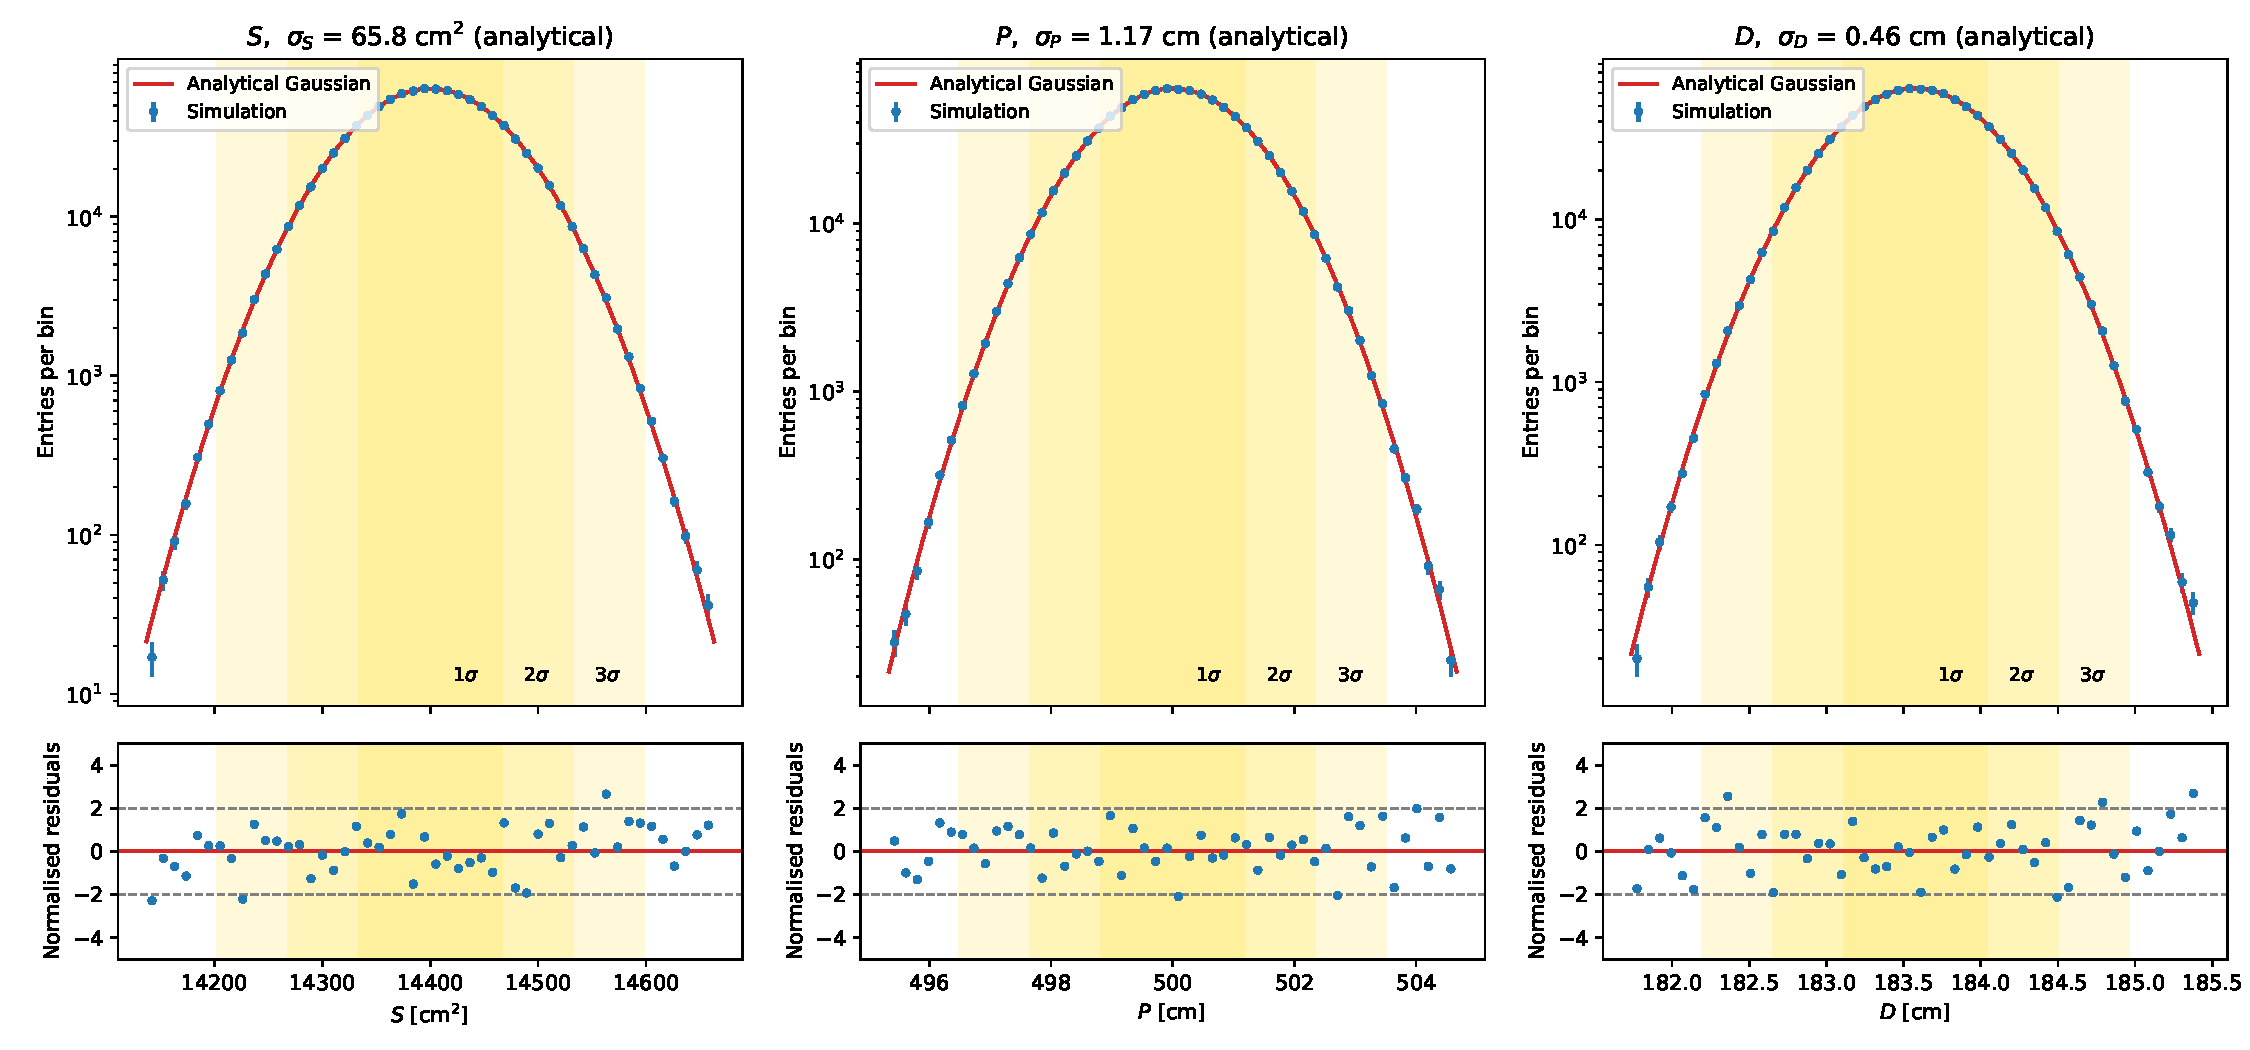
\includegraphics[width=\linewidth]{images/distributions.pdf}
		\caption{Top: distributions of the surface $S$, perimeter $P$ and diagonal $D$ of the $N = 10^6$ simulated tables (blue points), compared with the Gaussian distributions with the analytical standard deviations (red lines). The shaded bands highlight the regions within $\pm 1\sigma$, $\pm 2\sigma$ and $\pm 3\sigma$ from the nominal value. Bottom: normalised residuals; the dashed lines mark the $\pm 2$ range.}
		\label{fig:distributions}
	\end{figure}
	\FloatBarrier
	
	\section*{Result}
	
	The expected variations of the table surface, of the total length of the table sides and of the table diagonal, and the correlation between the surface and the total edge length, are reported in Table~\ref{tab:result}.
	
	\begin{table}[!h]
		\centering
		\begin{tabular}{l c c}
			\hline
			Quantity & Analytical & Numerical ($N = 10^6$) \\
			\hline
			$\sigma_S$   & $65.8$ cm$^2$ & $65.8$ cm$^2$ \\
			$\sigma_P$   & $1.17$ cm     & $1.17$ cm     \\
			$\sigma_D$   & $0.46$ cm     & $0.46$ cm     \\
			$\rho(S, P)$ & $0.962$       & $0.962$       \\
			\hline
		\end{tabular}
		\caption{Expected standard deviations of the surface, perimeter and diagonal of the table, and correlation between surface and perimeter, from the analytical error propagation and from the numerical experiment.}
		\label{tab:result}
	\end{table}
	\FloatBarrier
	
	The two approaches agree within the statistical precision of the simulation, confirming that, for the small production tolerances considered, the first order error propagation gives an accurate description of the variations of all the derived quantities.
	
\end{document}
